\documentclass[10pt,a4paper]{scrartcl}
\PassOptionsToPackage{table}{xcolor}
\usepackage[utf8]{inputenc}
\usepackage[T1]{fontenc}
\usepackage[ngerman]{babel}
\usepackage{microtype, multicol, marginnote, bera, parskip}
\usepackage{listings, amsmath, amssymb, graphicx, tikz, epic}
\usepackage{stmaryrd} %for lightning arrow
\usepackage{pstricks, pst-node, pst-tree, pdflscape}
\usepackage[babel=true]{csquotes}
\usepackage{placeins}
\tolerance=2000
\setcounter{secnumdepth}{0}
\usepackage[inner=2cm,outer=2cm,top=1.5cm,bottom=1.5cm,includeheadfoot]{geometry}
\usepackage{multirow}
\newcommand{\subExercise}[1]{\vspace{0.5em} \noindent{\bf #1)}}
\author{Michael Mardaus \and Andrey Tyukin}
\title{
\includegraphics[scale=0.2]{../logo_schriftzug}\\
Technische Informatik: Abgabe 4}

\begin{document}

\maketitle

\section*{Exercise 4.1 (Full adder from decoder)}

\vspace{1em}
\begin{figure}[h]
  \centering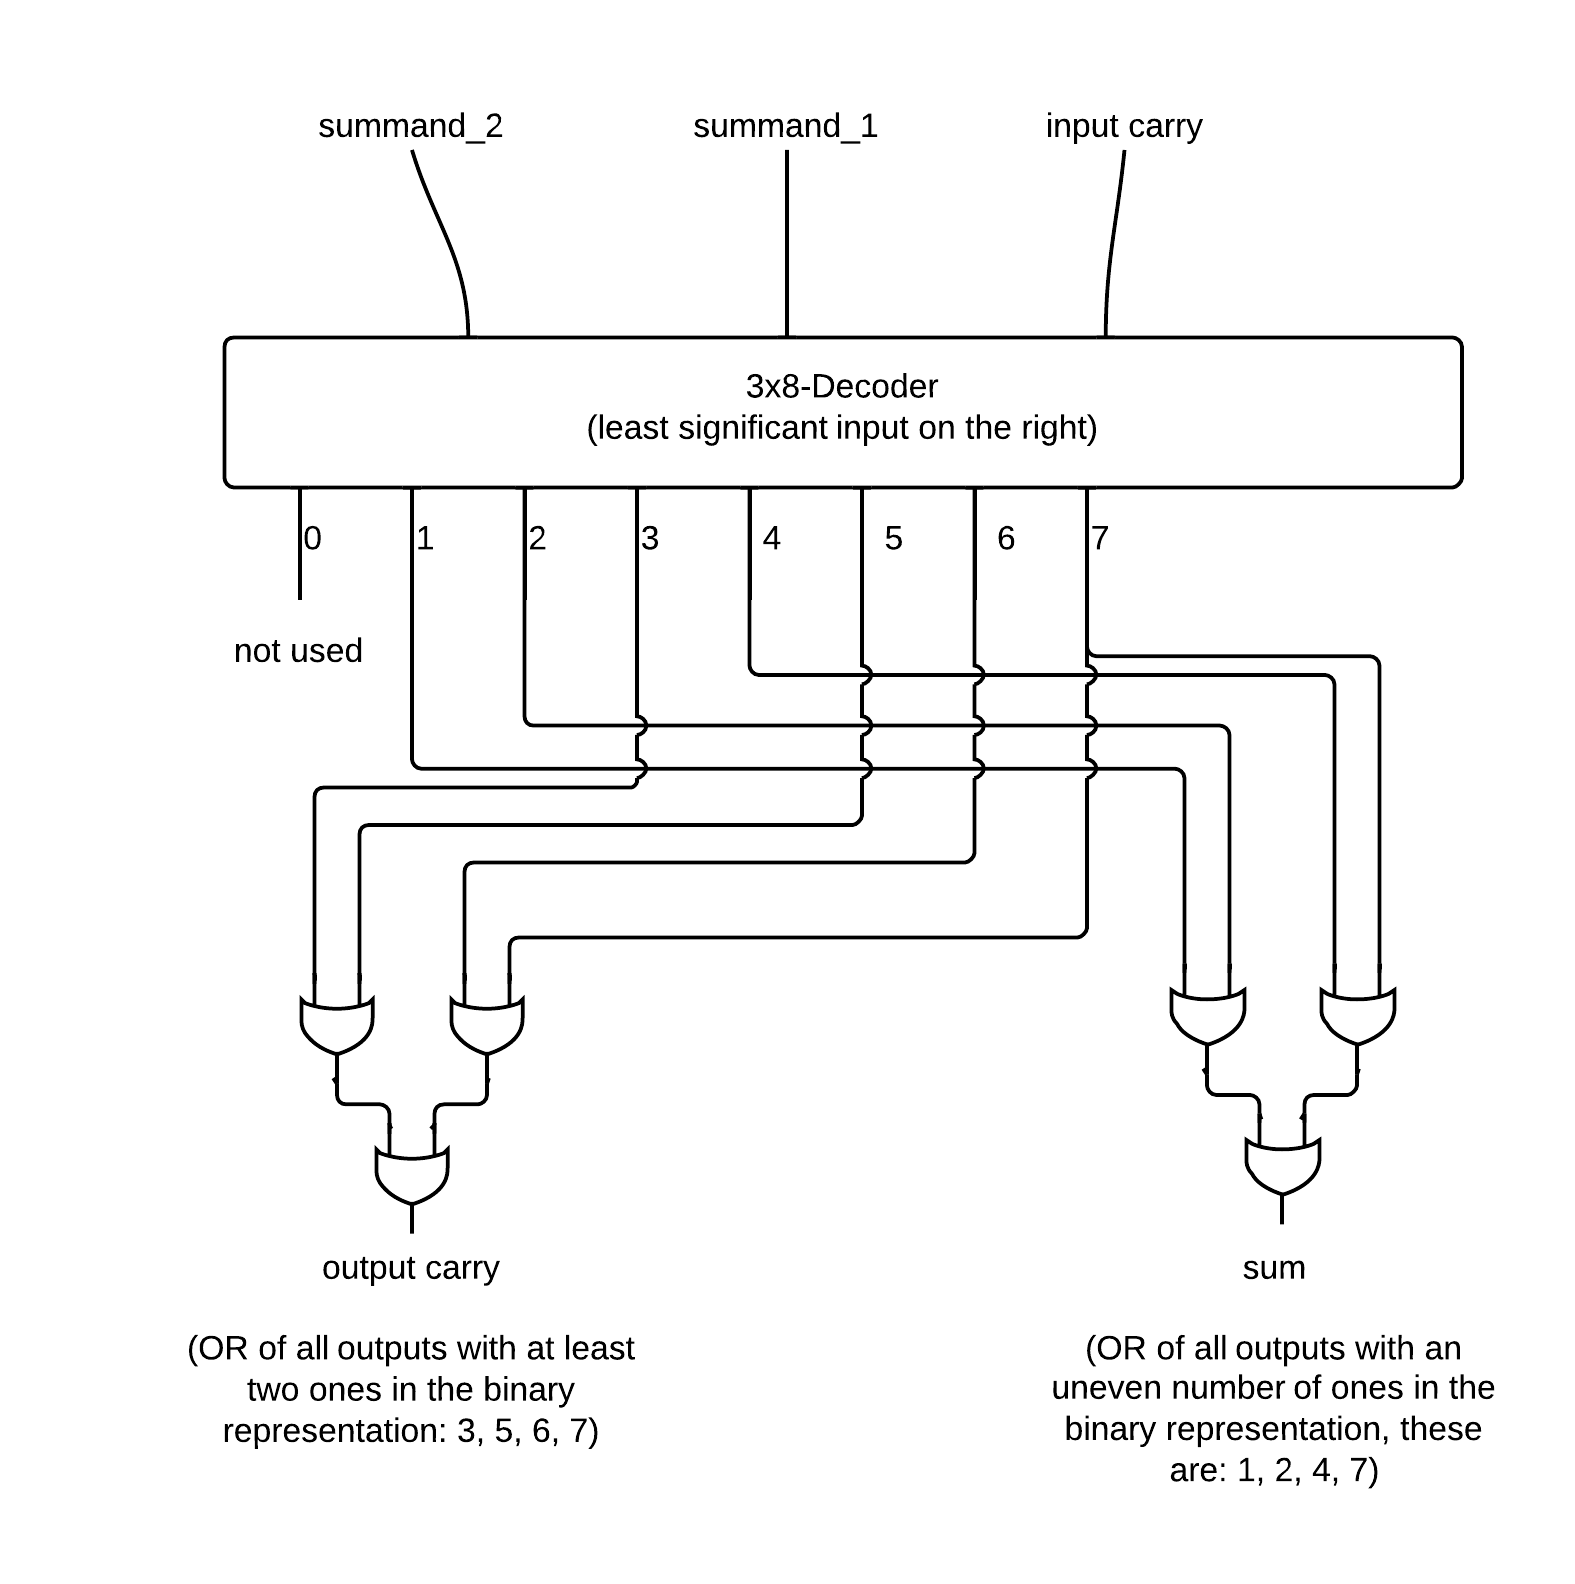
\includegraphics[width=0.6\linewidth]{images/fullAdder.png}
\end{figure}
\vspace{1em}

\FloatBarrier
\newpage
\section*{Exercise 4.2 (Subtractors)}
\subExercise{a}
Here are the tables for the two circuits we wish to implement 
(namely Half-Subtractor and Full-Subtractor):

\vspace{0.5em}
\begin{tabular}{|c c|c c|}
  \hline
  minuend & subtrahend & underflow & difference \\
  \hline
  0 & 0 & 0 & 0 \\
  0 & 1 & 1 & 1 \\
  1 & 0 & 0 & 1 \\
  1 & 1 & 0 & 0 \\
  \hline
\end{tabular}

\vspace{0.5em}
\begin{tabular}{|c c c|c c|}
  \hline
  minuend & subtrahend & underflow & underflow & difference \\
  \hline
  0 & 0 & 0 & 0 & 0 \\
  0 & 0 & 1 & 1 & 1 \\ 
  0 & 1 & 0 & 1 & 1 \\ 
  0 & 1 & 1 & 1 & 0 \\ 
  1 & 0 & 0 & 0 & 1 \\ 
  1 & 0 & 1 & 0 & 0 \\ 
  1 & 1 & 0 & 0 & 0 \\ 
  1 & 1 & 1 & 1 & 1 \\ 
  \hline
\end{tabular}

this is supposed to be a merge conflict
\subExercise{b} 
More or less compact symbolic representations 
of these two circuits are as follows 
(first component is always the resulting underflow, 
 second is the actual difference):
\[
  HalfSubtractor(m,s) = (\bar m s, m \not\leftrightarrow s)
\]
\[
  FullSubtractor(m,s,u) = 
    (\bar m \not\leftrightarrow su, 
     m \not\leftrightarrow s \not\leftrightarrow u
    )
\]
\subExercise{c} 
Now we want to simplify both components (difference and undeflow) 
of the full subtractor using Karnaugh diagrams. We begin with the
difference:

\vspace{0.5em}
\begin{tabular}{|c c|c c c c|}
  \hline 
    & & \multicolumn{4}{c|}{minuend / subtrahend} \\
    & & 00 & 01 & 11 & 10 \\
  \hline
    \multirow{2}{*}{underflow} & 0 & ? & ? & ? & ? \\
                               & 1 & \cellcolor{red}{?} & ? & ? & ? \\
  \hline
\end{tabular}
 
\subExercise{d}
\vspace{1em}
\begin{figure}[h]
  \centering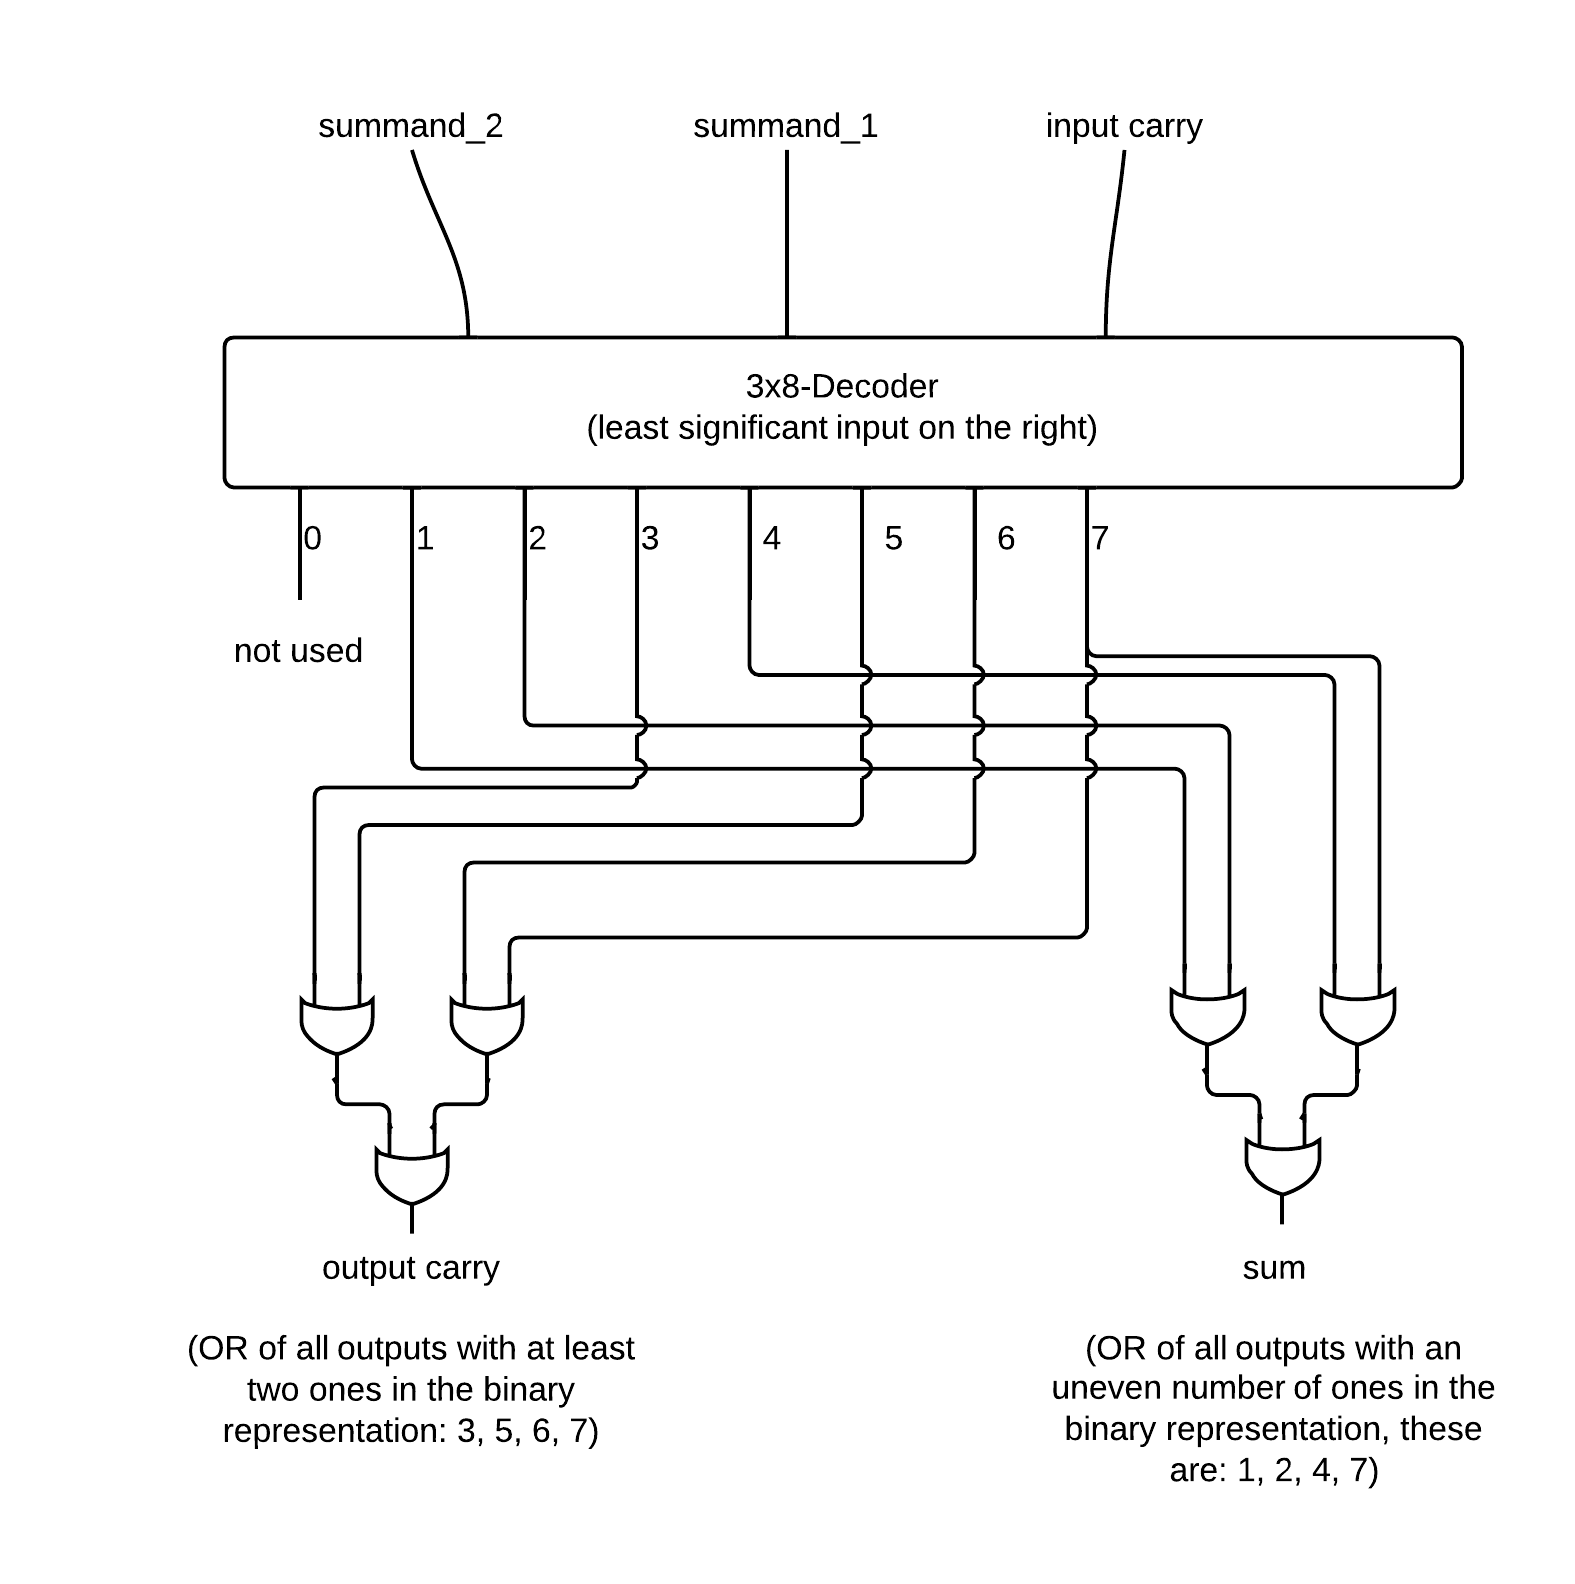
\includegraphics[width=0.6\linewidth]{images/fullAdder.png}
  \caption{Full subtractor. Notice that both outputs share some of the AND gates.}
\end{figure}
\vspace{1em}


\section*{Exercise 4.3 (TODO)}
\subExercise{a}
\subExercise{b}

\end{document}
